\documentclass[../monografia.tex]{subfiles}
\graphicspath{ {images/}{../images/} } 

\begin{document}
% Detalhar neste item os procedimentos realizados para os testes de funcionamento dos sub-sistemas, da inter-relação dos subsistemas e do sistema completo.
% \section{Verificação dos requisitos}

\section{Testes Realizados} %? Resultados dos Testes

\subsection{Validação dos Subsistemas} %? Testes Individuais
%Testes de funcionamento dos sub-sistemas

Para os sensores e o display, ao desenvolver cada uma das bibliotecas citadas na seção \ref{firmware}, também desenvolvemos exemplos para a validação de cada um individualmente. 

Utilizando a biblioteca de logging do ESP-IDF\cite{log-esp}, no modo Info, pudemos analisar os dados coletados pelos sensores, assim como os cálculos realizados, através do \textbf{IDF monitor}, uma ferramenta do ESP-IDF que funciona como um terminal serial, comunicando-se com o ESP32. 


% %? Problemas?
% Problema no MIC?


O sensor de luz \textbf{AS7262} tem como resposta 6 valores proporcionais à energia por unidade de área da luz incidente em cada espectro de seus filtros internos, de 450nm, 500nm, 550nm, 570nm, 600nm e 650nm. 

Para calcular a intensidade total da luz no ambiente fizemos alguns testes de calibração no LME com o técnico Carlos Ramos. Utilizando uma célula solar padrão com resposta conhecida, pudemos medir a intensidade real de uma luz branca incidindo sobre ela. Colomos em seguida o sensor AS7262 na mesma posição da célula, incidindo a mesma luz, com intensidade conhecida. 

Fizemos leituras com o sensor para diferentes intensidades, somamos os dados lidos pelo sensor para cada espectro e dividimos esse valor pelo tempo de integração configurado para a operação do sensor, conseguindo assim um valor proporcional à intensidade da luz. 
Com esses dados, mostrados na tabela \ref{tabela-luz}, foi possível encontrar uma constante calibrada para a conversão da leitura, em $\mu W/cm^2$. %?

%!! tabelas do teste de luz

\subsection{Validação do Dispositivo} %? Teste Completo

% \subsubsection{Montagem Final}

Com todos os subsistemas citados anteriormente validados, fabricamos uma PCB em uma fresa CNC e um case utilizando uma impressora 3D. Com isso, fizemos a montagem de um primeiro protótipo, como mostrado na figura \ref{fig:montagem-final}. 

\begin{figure}[h]
	\centering
	\begin{subfigure}{0.5\textwidth}
		\centering
	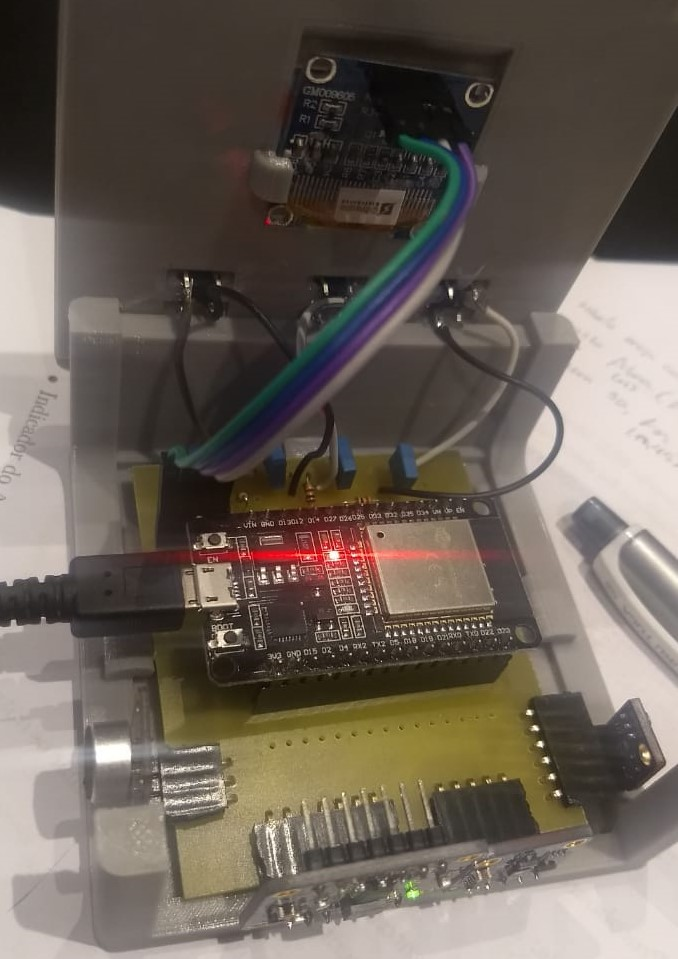
\includegraphics[width=0.8\textwidth]{placa-final}
	\caption{Interna}
	\label{fig:interna}
	\end{subfigure}%
	\begin{subfigure}{0.5\textwidth}
		\centering
		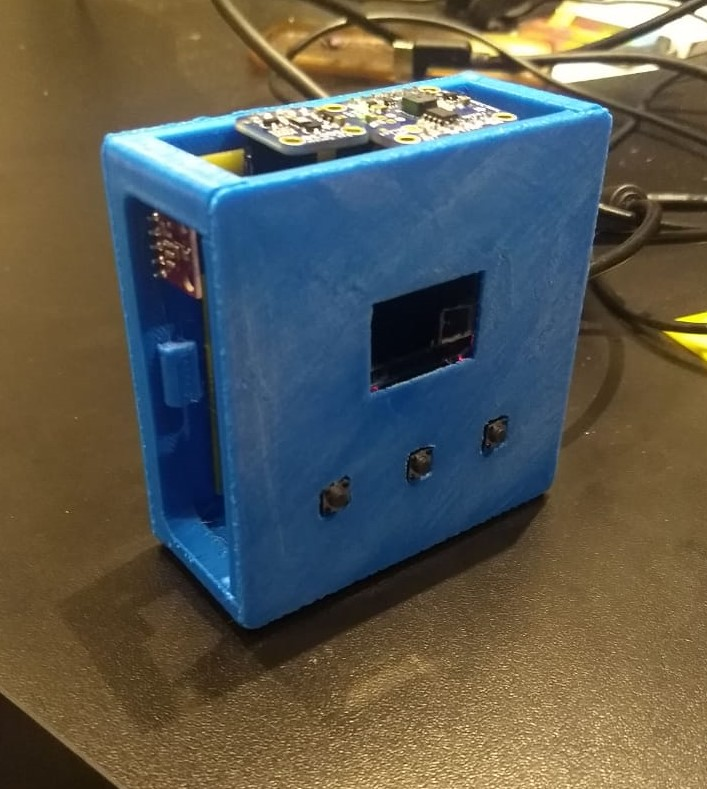
\includegraphics[width=\textwidth]{montagem-final.jpg}
		\caption{Externa}
		\label{fig:externa}
	\end{subfigure}
	\caption{Montagem final do dispositivo}
	\label{fig:montagem-final}
\end{figure}

Para validação de cada subcircuito presente na PCB, utilizamos os mesmos exemplos citados para validação dos sensores e do display, até então testados usando uma protoboard de testes.

Com o firmware completo desenvolvido, fizemos testes com um só dispositivo, utilizando a mesma biblioteca de Log e o IDF monitor. Os dados dos quatro sensores operando em paralelo podem ser vistos na figura \ref{fig:monitor-sensors}.

%! monitor com dados sensores
\begin{figure}[h]
	\centering
	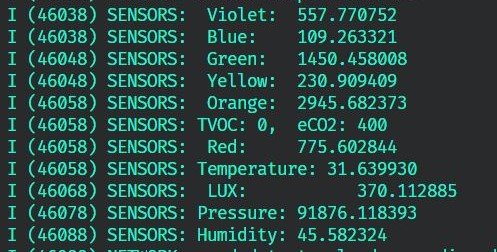
\includegraphics[width=\textwidth]{monitor-sensors}
	\label{fig:monitor-sensors}
	\caption{Coleta dos sensores no IDF-Monitor}
\end{figure}

Em seguida, incluímos o envio dos dados via WiFi, como citado em \ref{dev-Wi-Fi}, com o dispositivo operando como gateway. Os dados das coletas, agora salvos no banco de dados, foram apresentados no dashboard como mostra a figura \ref{fig:dashboard-graphs}.

\begin{figure}[h]
	\centering
	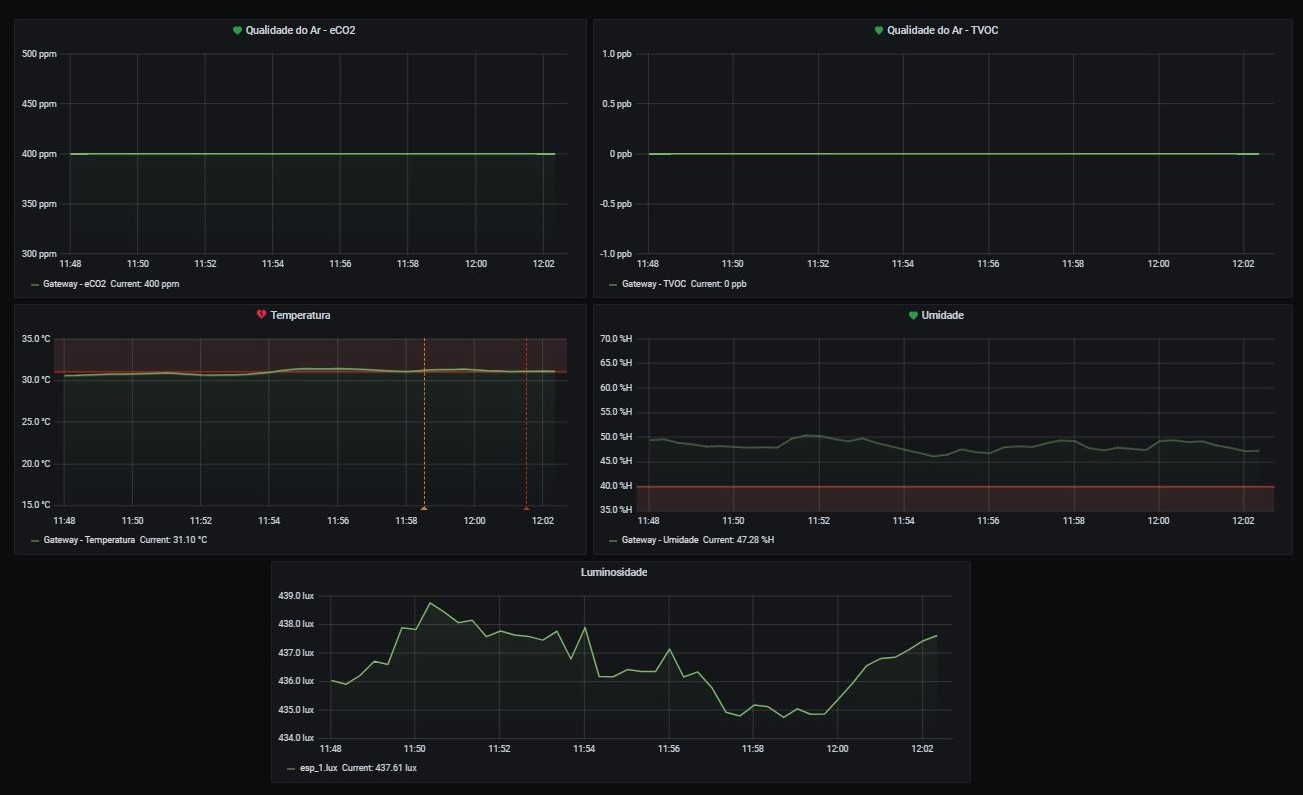
\includegraphics[width=\textwidth]{dashboard-graphs}
	\label{fig:dashboard-graphs}
	\caption{Gráficos de coletas do Gateway no Dashboard}
\end{figure}

Fabricamos mais dois dispositivos para criar então a rede completa, utilizando BLE-Mesh e um dos 3 funcionando como Gateway para enviar os dados para o dashboard. 

\begin{figure}[h]
	\centering
	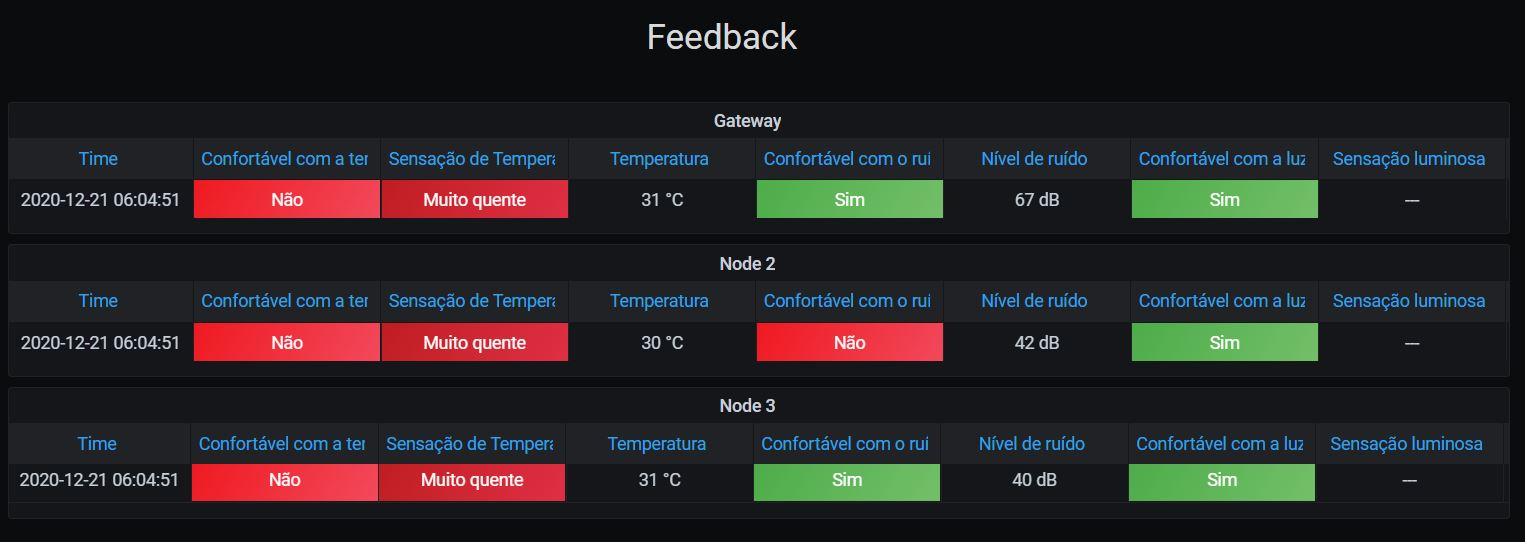
\includegraphics[width=\textwidth]{dashboard-feedback}
	\label{fig:dashboard-feedback}
	\caption{Feedbacks no Dashboard}
\end{figure}

\begin{figure}[h]
	\centering
	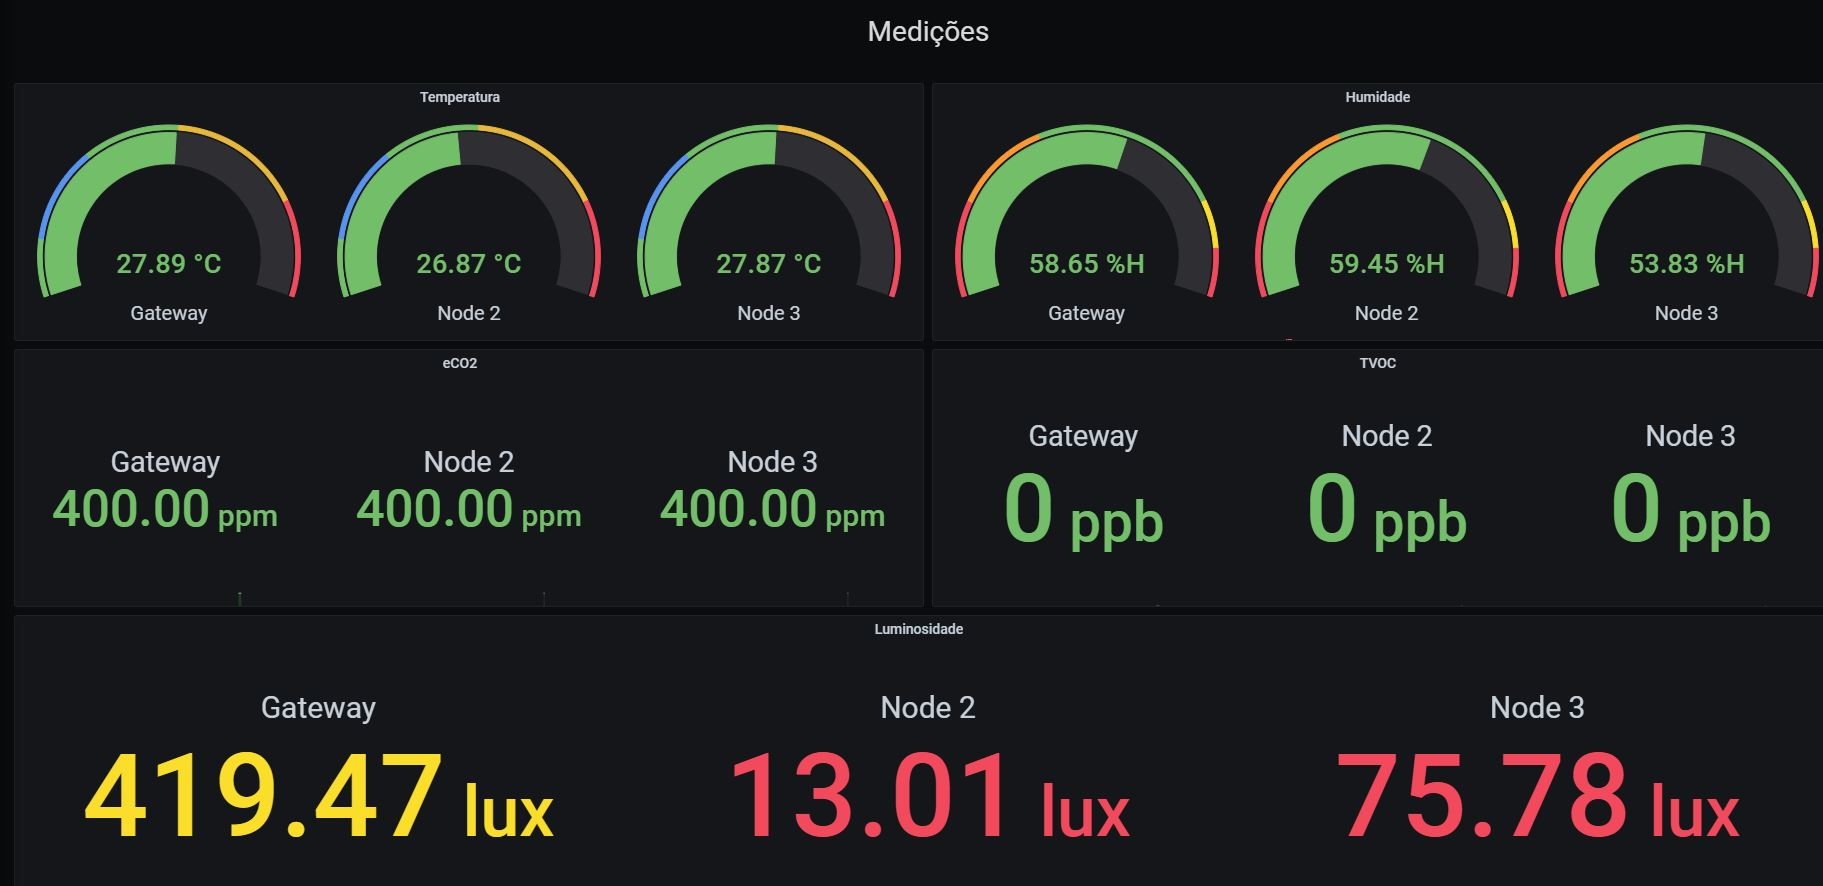
\includegraphics[width=\textwidth]{dashboard-medicoes}
	\label{fig:dashboard-medicoes}
	\caption{Últimas medições dos indicadores no Dashboard}
\end{figure}

\end{document}